\documentclass{article}%ctex
\input{~/code/math_commands.tex}




\title{\huge Session 7\\
\normalsize}
\author{Xuanxi Zhang}
\begin{document}
\maketitle
\section{Householder reflectors}
\subsection{review}
\begin{itemize}
    \item $P$ is called a projector if $P^2 = P$. Check $P_v=\frac{vv^T}{v^Tv}$ is a projector onto the line spanned by $v$.
    \item If $\text{range}\{P\}$ is orthogonal with $\text{range}\{I-P\}$, then $P$ is called an orthogonal projector. For a projector $P$, it is an orthogonal projector if and only if $P^T=P$. Check $P_v$ is an orthogonal projector. 
    \item Householder Transform $H_v=I-2\frac{vv^T}{v^Tv}=(I-P_v)-P_v$. Check $H_v$ is an orthogonal matrix.
    \item A orthogonal matrix doesn't change the length of a vector. Mathematcially, $\norm{Qx}_2=\norm{x}_2$, where $Q$ is an orthogonal matrix.
\end{itemize}


\subsection{Geometric interpretation of Householder reflectors}
We aim to apply the Householder transformation to map a vector \( x \) to \( c e_1 \), where \( e_1 \) is the first standard basis vector. Since the Householder transformation is an orthogonal matrix, it preserves the length of vectors, implying \( c = \pm \|x\|_2 \). We arbitrarily choose \( \|x\|_2 e_1 \). In the following figure, both the vectors \( x \) and \( \|x\|_2 e_1 \) are already marked. To construct the Householder vector, we define \( v = \|x\|_2 e_1 - x \), which is also shown in the figure, pointing from \( x \) to \( \|x\|_2 e_1 \).

Plot \( P_v x \), \( (I - P_v) x \), and \( -P_v x \) in the figure, where \( P_v \) is the projection matrix defined above. Verify that the Householder transformation satisfies \( (I - 2P_v) x = \|x\|_2 e_1 \).


\begin{figure}[H]
    \centering
    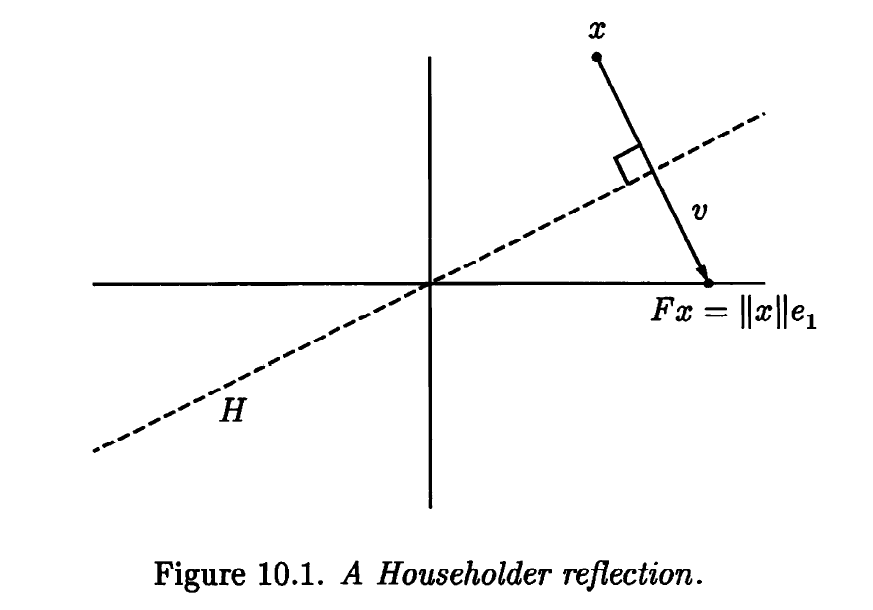
\includegraphics[width = 0.4\textwidth]{./1.png}
\end{figure}

\subsection{a more general case}
If I want to reflect $x$ to align with $y$ using an orthogonal matrix, what will the resulting vector be? What is the corresponding Householder reflector?



\section{IEEE 754 Standards}
The IEEE 754 standard defines floating-point representations for higher precision, commonly using 32-bit (single precision) and 64-bit (double precision) formats. Floating-point numbers are represented in scientific notation. In binary, this takes the form:
$$
\pm 1.M \times 2^E
$$
where \( M \) is the mantissa and \( E \) is the exponent.

IEEE 754 Single Precision (32-bit) uses the following format: 1 bit for the sign, 8 bits for the exponent, 23 bits for the mantissa.

IEEE 754 Double Precision (64-bit) uses the following format: 1 bit for the sign, 11 bits for the exponent, 52 bits for the mantissa.


Now, let's consider a simplified 8-bit floating-point system:
\begin{itemize}
    \item 1 bit for sign. 0 for positive, 1 for negative.
    \item 3 bits are allocated for the exponent. In order to represent both positive and negative exponents, a bias is added to the actual exponent. The bias is chosen to be \(2^{(n-1)} - 1\), where \(n\) is the number of bits allocated for the exponent. In our case, the bias is 3. For example, if the actual exponent is -1, the stored exponent will be 2 in decimal and 010 in binary. Usually all 1s and all 0s are reserved for special cases.
    \item 4 bits are allocated for the mantissa. If we use binary scientific notation, the first digit of the this part is always 1, so we can only represent the mantissa.
\end{itemize}

\subsection{}
Represent the number \(6.25\) in this 8-bit floating-point system. 

\subsection{}
Try to represent \(-3.5\) in the same 8-bit floating-point system.

\subsection{}
What is the largest number that can be represented in this 8-bit system? To make it the biggest, we should choose sign to be positive, which is 0. And then choose exponent to be the biggest, which is 110.(note that 111 is reserved). And then choose mantissa to be the biggest, which is 1111. So the biggest number in our 8 bit system is \(0 \, 110 \, 1111\). Convert it to decimal number. 

\subsection{}
Check \(0\,001\,0000\) is the smallest positive number in our 8 bit system. Convert it to decimal number.

\subsection{comments}
Note that the largest number for single precision is \(3.4028235 \times 10^{38}\), and the smallest positive number is \(1.17549435 \times 10^{-38}\). The largest number for double precision is \(1.7976931348623157 \times 10^{308}\), and the smallest positive number is \(2.2250738585072014 \times 10^{-308}\). These formats allow for much greater precision and a wider range of values than the simplified 8-bit system, enabling modern computers to handle complex calculations efficiently.

\begin{figure}[H] 
\centering 
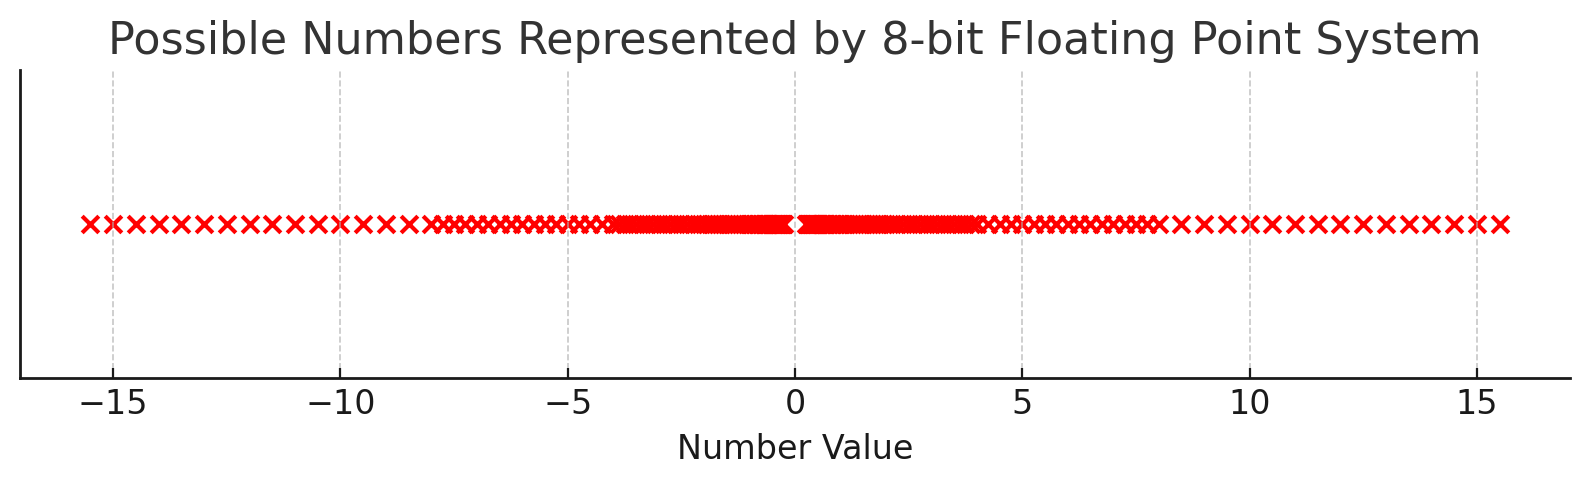
\includegraphics[width=0.7\textwidth]{./output.png}
\caption{This figure shows all possible 8-bit floating-point numbers. All floating-point number representation systems share a similar property: numbers are denser near 0 and become sparser as they approach the largest representable values}
\end{figure}


\section{Intro to Power method}
Suppose \( A \) is a symmetric matrix with $n$ different eigenvalues, $|\lambda_1|>|\lambda_2|>\cdots>|\lambda_n|$ and corresponding eigenvectors $v_1,v_2,\cdots,v_n$. Then for any vector $x$, we can decompose it as $x=\sum_{i=1}^n c_i v_i$, where $c_i=x^Tv_i$. Since $A^kx=\sum_{i=1}^n\lambda_i^k c_i v_i$, if $c_1$ is not zero, then $\frac{A^kx}{\lambda_1^k}\to c_1v_1$ as $k\to\infty$. This is the idea of power method.

    


\end{document}



